\documentclass{scrartcl}
 
\usepackage[utf8]{inputenc}
\usepackage[T1]{fontenc}
\usepackage{lmodern}
\usepackage[pdftex]{graphicx}
\usepackage[ngerman]{babel}
\usepackage{amsmath}
\usepackage{tabularx}
\usepackage{multirow}
\usepackage{amsfonts}
\usepackage{tabto}
\TabPositions{0.1in, 0.4in, 0.6in, 0.8in, 1.0in, 1.2in, 3.4in}

\begin{document}
\begin{LARGE}
Spieltheorie - WiSe 2014/15
\end{LARGE}

\begin{Large}
Übungsblatt 1 - Felix Dosch\\[1.0cm]
\end{Large}

\begin{Large}
Aufgabe 1\\[0.0cm]
\end{Large}

a) Die Extensivform des beschriebenen Spiels lautet: $\Gamma = (N, V, E, r, (V_i)_{i \in N}, O, u)$ mit

\begin{itemize}
\item{$N = \{A, P\}$}
\item{$V = \{r, a, b, c, d, e, f, g\}$}
\item{$E = \{(r, a), (r, b), (r, c), (b, d), (b, e), (c, f), (c, g)\}$}
\item{$V_A = \{r\}$}
\item{$V_P = \{b, c\}$}
\item{$O = \{(0\$, 0\$), (2000\$, 2000\$), (7000\$, -3000\$)\}$}
\item{$u(a) = u(e) = u(g) = (0\$, 0\$), u(d) = (2000\$, 2000\$), u(f) = (7000\$, -3000\$)$}
\item{Aktionen in r: 1 - Nicht anbieten, 2 - Anbieten für 10000\$, 3 - Anbieten für 15000\$}
\item{Aktionen in b: 1 - Annehmen, 2 - Ablehnen}
\item{Aktionen in c: 1 - Annehmen, 2 - Ablehnen}
\end{itemize}
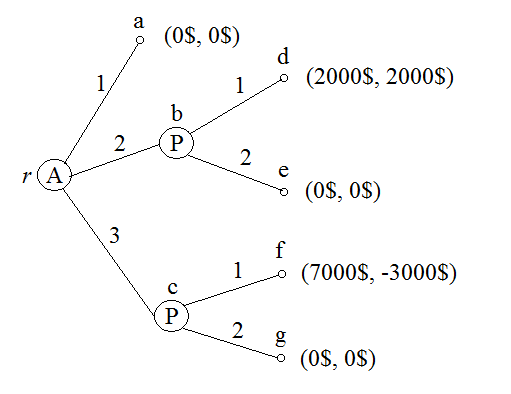
\includegraphics[width=10.5cm]{spielbaum_1a_fertig.png} \\

b) Die Extensivform des beschriebenen Spiels lautet: $\Gamma = (N, V, E, r, (V_i)_{i \in N}, O, u)$ mit

\begin{itemize}
\item{$N = \{I, II\}$}, wobei $I$ = Mrs. Smith und $II$ = Mr. Smith
\item{$V = \{r, a, b, c, d, e, f\}$}
\item{$E = \{(r, a), (r, b), (a, c), (a, d), (b, e), (b, f)\}$}
\item{$V_I = \{r\}$}
\item{$V_{II} = \{a, b\}$}
\item{$O = \{(0\$, 0\$), (100\$, 100\$)$}
\item{$u(d) = u(e) = (0\$, 0\$), u(c) = u(f) (100\$, 100\$)$}
\item{Aktionen: 1 - Gehe zu Empire State Building, 2 - Gehe zu Freiheitsstatue}
\end{itemize}
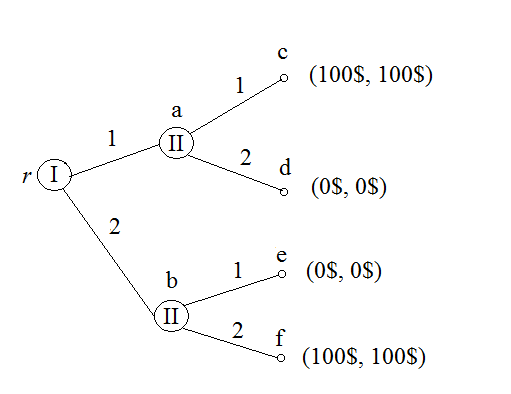
\includegraphics[width=14.5cm]{spielbaum_1b.png} \\



\clearpage
\begin{Large}
Aufgabe 1.2\\[0.0cm]
\end{Large}

a) Der schwarze Spieler ($II$) besitzt eine Gewinnstrategie. Diese beruht im Wesentlichen auf der Tatsache, dass
er auf die Züge von Weiß ($I$) reagieren kann, und dadurch das Spiel immer wieder in ein "Gleichgewicht"
bringen
kann, indem er wie das Spiegelbild von Weiß zieht. Dies ist intuitiv immer möglich, sofern Schwarz von Beginn
an immer diesen Zug macht, wobei sich jedes
Bauernpaar in der Mitte des Brettes (4- und 5-Linie) trifft, wobei Schwarz immer den letzten Zug auf die 5-
Linie macht, und damit im Falle des letzten Bauernpaares kein Zug für Weiß bleibt, womit Weiß verliert.

Da Weiß beginnt, hat jeder Knoten $C(x)$, bei dem Schwarz am Zug ist einen Vaterknoten $x$ und eine Aktion
$A(x)$ in der Form "$y$-Bauer $k$ Felder vor". Dabei bezeichne $y$ eine der Reihen A bis H. Die Antwort auf
diesen Zug ist jeweils genau der entgegengesetzte Zug, also auch "$y$-Bauer $k$ Felder vor".

Sei $M$ die Menge aller Knoten, bei denen sich auf dem Brett eine symmetrische Bauernaufstellung ergibt, d.h.
es gilt für alle $y \in \{A, B, ..., G, H\}$ und alle $i \in \{1, 2, 3, ..., 7, 8\}$:
Weißer Bauer auf $yi \Leftrightarrow$ Schwarzer Bauer auf $y(9-i)$.

Somit ist folgendes eine Gewinnstrategie für Schwarz: \newline

\[ \forall x \in V_{II}\text{ : }s_{II}(x) = \left\{
\begin{array}{l l}
(x, z) \text{, mit }x = C(y) \text{ und } z \in M & \quad \text{falls } y \in M\\
(x, p) & \quad \text{sonst}
\end{array} \right.\] 

Hierbei soll $p$ die Situation sein, die entsteht wenn $II$ den linkesten beweglichen Bauern
ein Feld vor zieht.

Solange Weiß an einem Knoten aus $M$ ist, kann Schwarz immer so reagieren, dass Weiß wieder an einem Knoten aus
$M$ ist. Mit dieser Invariante gelangt Schwarz bis zum letzten möglichen Zug, nach welchem alle weißen Bauern
auf der 4-Reihe und alle schwarzen Bauern auf der 5-Reihe stehen, wo Weiß keine Zugmöglichkeit mehr hat.\newline

b) Wenn Schwarz beginnt ist das wie ein Farbtausch von Weiß und Schwarz. Entsprechend hat dann Weiß eine
Gewinnstrategie.

\clearpage
\begin{Large}
Aufgabe 1.3\\[0.0cm]
\end{Large}

a) Die Idee ist es, einen Spielbaum zu haben, bei dem sich für Blätter auf gleicher Ebene (gleiche Entfernung zur
Wurzel) entlang des Pfades die gleiche Gesamtwahrscheinlichkeit ergibt. Der Baum wiederholt sich in sich selbst,
da das Spiel dann quasi wieder von vorne beginnt, da bisher keine Entscheidung gefunden werden konnte.

Der Algorithmus läuft wie folgt ab:
\begin{itemize}
\item{1. Werfe die Münze und merke das Ergebnis $x$}
\item{2. Werfe die Münze erneut und merke das Ergebnis $y$}
\item{3. Falls $x \neq y$ : $y$ gewinnt. Ansonsten gehe zu 1.}
\end{itemize}

Hiermit wird eine faire Münze simuliert, da die Wahrscheinlichkeit für Kopf-Zahl und Zahl-Kopf in zwei
hintereinanderfolgenden Würfen immer genau gleich ist (Kommutativität: $p \cdot (1-p) = (1-p) \cdot p$). In den
anderen Fällen wird das Spiel wieder von vorne begonnen und die Wahrscheinlichkeit zu gewinnen ist wieder für
beide gleich.


\end{document}

